\subsection{Imagen Fantasma}
Este filtro consiste en generar una imagen fantasma utilizando parte de la imagen original en escala de grises y al doble de su tamaño. La parte utilizada será de tamaño ancho/2 x alto/2, y se pasará por parámetro un offset en x e y, que determinará cuál será la imagen fantasma. Cabe aclarar que el rango de los offsets están entre 0 y ancho/2 +1. Si no se pasa ningún offset, el predeterminado es 0, si se pasa algún valor fuera de rango se utilizará el máximo o mínimo offset según corresponda.

\subsubsection{Pseudocódigo del ciclo:}
\begin{codesnippet}
\begin{verbatim}
Para i de 0 a height - 1;
    Para j de 0 a width - 1; 
        int ii = i/2 + offsetY;
        int jj = i/2 + offsetX;
        float b = (src_matrix[ii][jj].r + 2 * src_matrix[ii][jj].g + src_matrix[ii][jj].b) / 4;
        dst_matrix[i][j].r = SATURAR(src_matrix[i][j].r * 0.9 + b/2);
        dst_matrix[i][j].g = SATURAR(src_matrix[i][j].g * 0.9 + b/2);
        dst_matrix[i][j].b = SATURAR(src_matrix[i][j].b * 0.9 + b/2);
\end{verbatim}
\end{codesnippet}

\subsubsection{Implementación del ciclo en ASM}
Como este filtro opera con todos los pixeles, se recorren desde el primer al último pixel de las imágenes de a dos pixeles por ciclo. Paralelamente voy recorriendo la submatriz fantasma de a un pixel por ciclo, con la ayuda de un registro que contendrá la dirección de memoria correspondiente al \textbf{offsetX} e \textbf{offsetY}. 
Pero a diferencia de la matriz fuente y destino, en la submatriz fantasma las filas se recorren dos veces consecutivamente. \\
Adicionalmente se declaran en memoria los siguientes datos floats que para realizar los cálculos necesarios: 
\begin{codesnippet}
\begin{verbatim}   
    mul09:  dd 0.9, 0.9, 0.9, 1.0 
    calc_b: dd 1.0, 2.0, 1.0, 0.0 
    div8:   dd 8.0, 8.0, 8.0, 8.0 
\end{verbatim}
\end{codesnippet}

{\centering\textbf{Cálculo de b/2:}}

Se carga en un registro \textbf{XMM} el pixel apuntado de la submatriz fantasma, es decir leo 4 bytes. \\
Se desempaqueta dos veces la parte baja del registro, es decir el pixel pasó de tener 4 componentes de 1 byte, a 4 componentes de 2 bytes y luego pasasaron a ser de 4 bytes, para convertirlos al tipo float. \\
El siguiente paso es multiplicar el registro por la máscara [calc\_b] para dejar la transparencia en 0 momentáneamente y tener el doble valor de la componente G. \\
Luego se realizan dos sumas horizontales, sobre el mismo registro, obteniendo 4 floats con el mismo valor como se puede ver en la figura~\ref{sumah}. \\
Luego se shiftea 4 bytes a la derecha para dejar en 0's el último float, que se corresponde con tener la transparencia en 0.
Finalmente se divide el registro por [div8], finalizando el cálculo de b y representando lo siguiente:
\begin{codesnippet}
\begin{verbatim}
        XMM = |0|b/2|b/2|b/2|;
\end{verbatim}
\end{codesnippet}

\begin{figure}[h]
  \begin{center}
	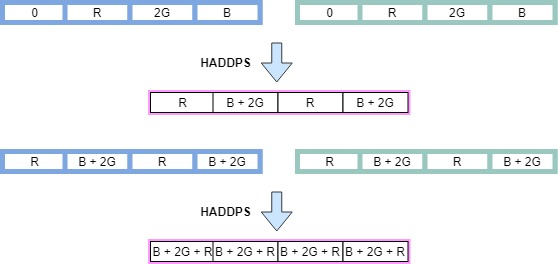
\includegraphics[scale=0.5]{img/haddps.jpg}
	\caption{Diagrama de operar con la instrucción HADDPS}
	\label{sumah}
  \end{center}
\end{figure}

{\centering\textbf{Procesado de los pixeles [i][j] y [i][j+1]:}}

Se cargan en un registro\textbf{XMM} 2 pixeles (8 bytes) de la imagen \textbf{src}.
Se desempaqueta la parte baja de byte a word, luego se guarda una copia del registro, y se desempaqueta cada componente de word a doubleword, sólo que para un registro la parte baja y para el otro la parte alta. \\
Obteniendo los valores de los componentes del pixel [i][j] en un registro y los de [i][j+1] en el otro. Y se convierten a float. \\
Luego se multiplica cada uno por los valores de \textbf{[mul09]}. 
Y se suma el registro que contiene 4 floats con el valor b/2 previamente calculado. \\
Luego se convierten los registros a datos enteros, se empaquetan a word y luego a byte sin signo y con saturación, obteniendo los valores esperados. \\
Finalmente se escriben en la imagen \textbf{dst}.
\begin{codesnippet}
\begin{verbatim}
        dst_matrix[i][j].r = SATURAR(src_matrix[i][j].r * 0.9 + b/2);
        dst_matrix[i][j].g = SATURAR(src_matrix[i][j].g * 0.9 + b/2);
        dst_matrix[i][j].b = SATURAR(src_matrix[i][j].b * 0.9 + b/2);
\end{verbatim}
\end{codesnippet}
\begin{figure}[ht]
  \begin{center}
	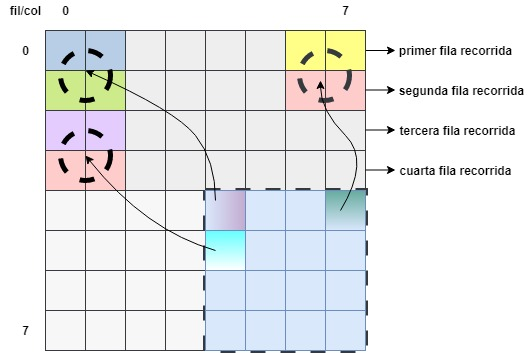
\includegraphics[scale=0.5]{img/fantasma1.jpg}
	\caption{Representación parcial de aplicar b/2 a cada pixel con el máximo valor de offset de X e Y}
	\label{calcb}
  \end{center}
\end{figure}

Llegando al final del ciclo, se avanzan los punteros dos pixeles de las imágenes \textbf{src} y \textbf{dst}, se evalúan los saltos condicionales para saber si ya no quedan pixeles por procesar, o si se continúa pero cambiando la fila de la matriz fantasma o si se vuelve al inicio de esta.

\newpage